\begin{figure*}[!ht]
	\centering{
		\hspace*{\fill}
		\begin{subfigure}{0.4\textwidth}
			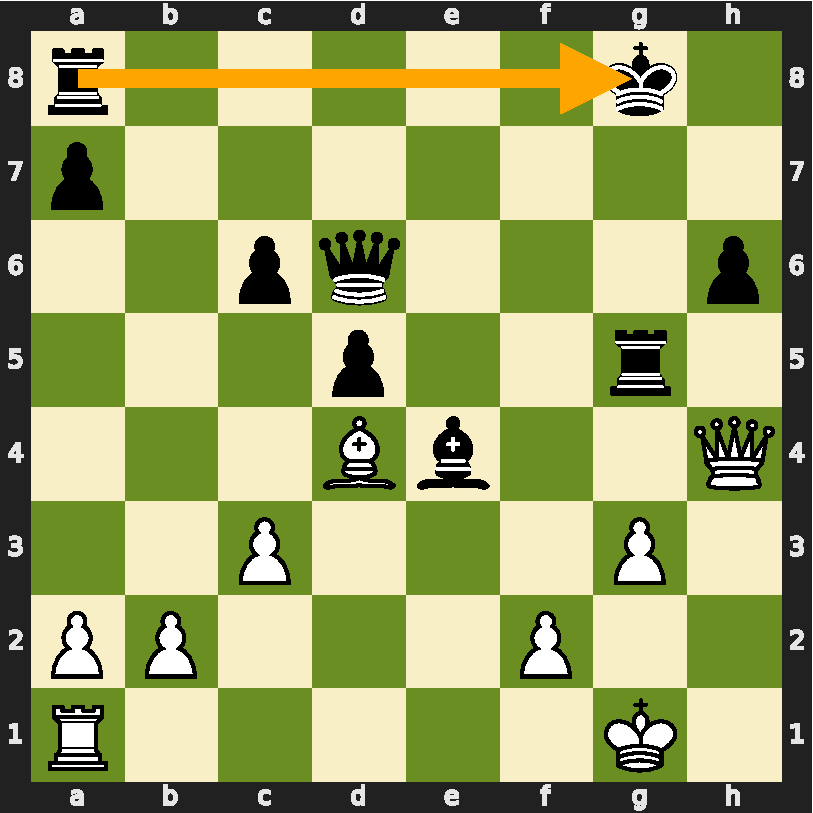
\includegraphics[width=\linewidth]{figures/board_path_rook.pdf}
			\caption{Rook forgets about its own king at \pos{g8}!} 
			\label{fig:rook_path}
		\end{subfigure}
		\hspace*{\fill}
		\begin{subfigure}{0.4\textwidth}
			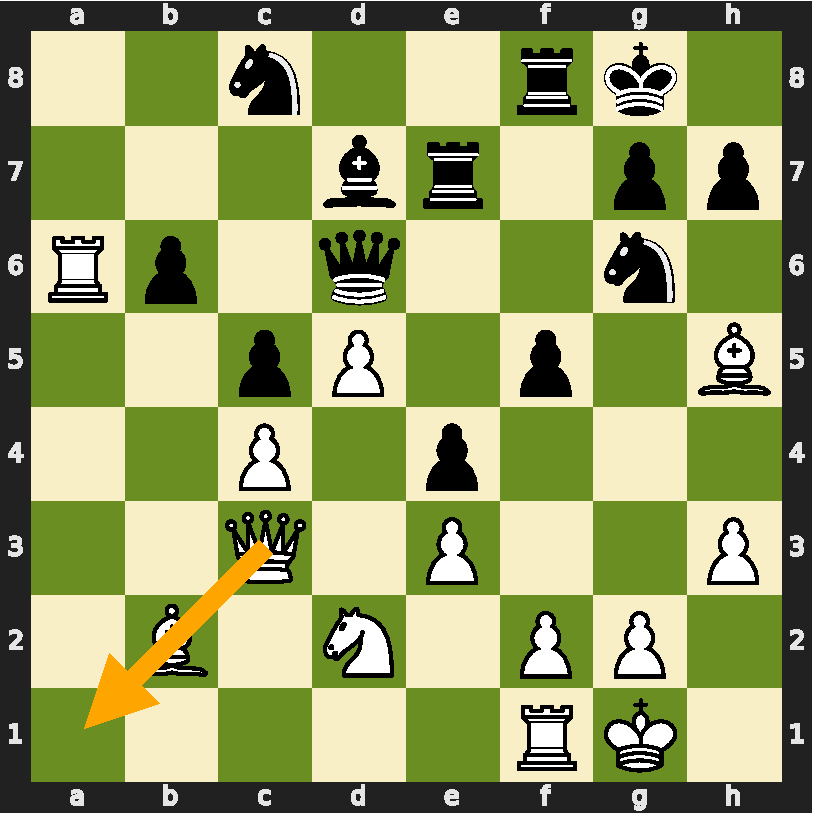
\includegraphics[width=\linewidth]{figures/board_path_queen.pdf}
			\caption{Bishop at \pos{b2} stands in the way of the queen.} 
			\label{fig:queen_path}
		\end{subfigure}
		\hspace*{\fill}
		\\[1em]
		\hspace*{\fill}
		\begin{subfigure}{0.4\textwidth}
			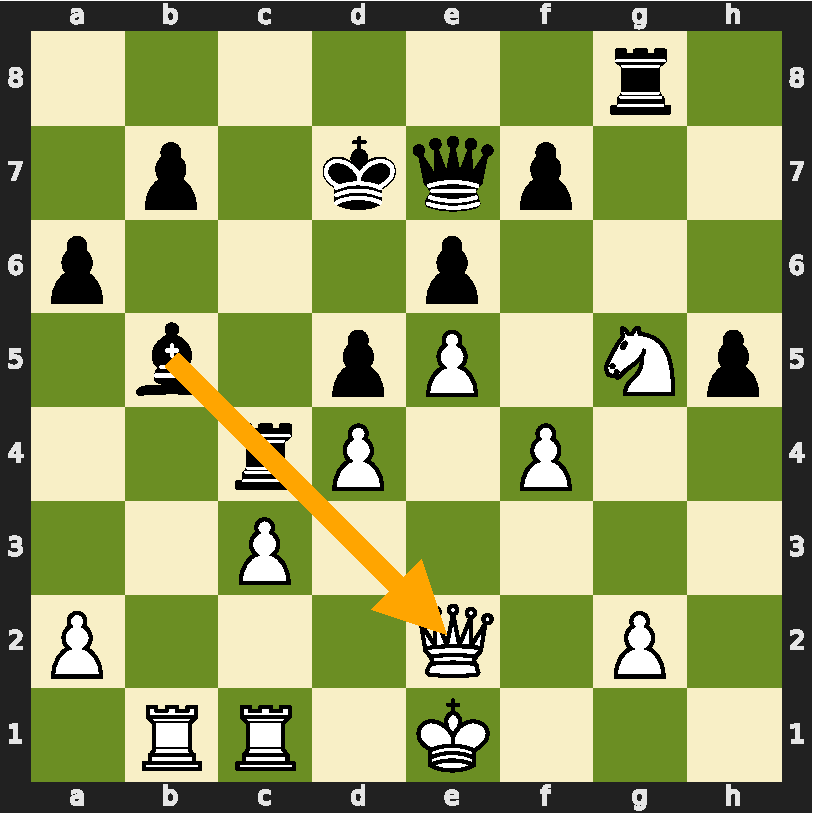
\includegraphics[width=\linewidth]{figures/board_path_bishop.pdf}
			\caption{Bishop forgets reality in pursuit of fantasy queen kill!} 
			\label{fig:bishop_path}
		\end{subfigure}
		\hspace*{\fill}
		\begin{subfigure}{0.4\textwidth}
			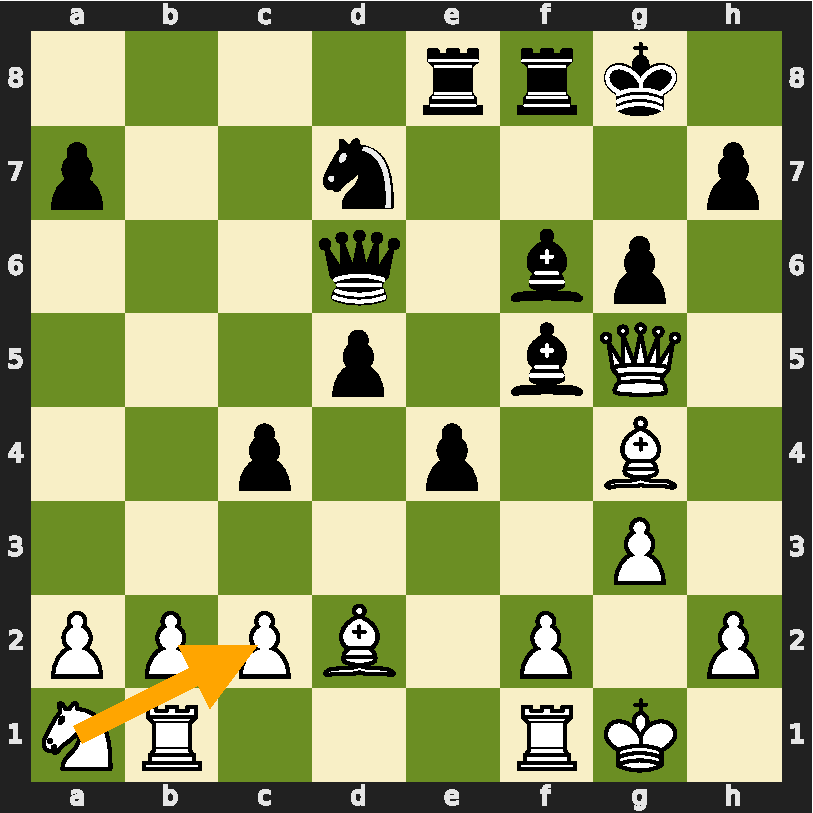
\includegraphics[width=\linewidth]{figures/board_path_knight.pdf}
			\caption{A trapped, frustrated knight is out to kill its own pawn!} 
			\label{fig:knight_path}
		\end{subfigure}
		\hspace*{\fill}
		\caption{Instances of Path Obstruction errors with different piece types.}
		\label{fig:path_obstruction}
	}
\end{figure*}


\begin{figure*}[!ht]
	\centering{
		\hspace*{\fill}
		\begin{subfigure}{0.35\textwidth}
			\includegraphics[width=\linewidth]{figures/path_obs_actual.jpg}
			\caption{End-Actual} 
			\label{fig:path_length_actual}
		\end{subfigure}
		\hspace*{\fill}
		\begin{subfigure}{0.35\textwidth}
			\includegraphics[width=\linewidth]{figures/path_obs_other.jpg}\\
			\caption{End-Other} 
			\label{fig:path_length_other}
		\end{subfigure}
	\hspace*{\fill}
\caption{Comparison of average path length of predicted moves for different piece types when the move is legal vs ones with path obstruction error.}
\label{fig:path_length}
}
\end{figure*}